\begin{figure}[h]
\centering
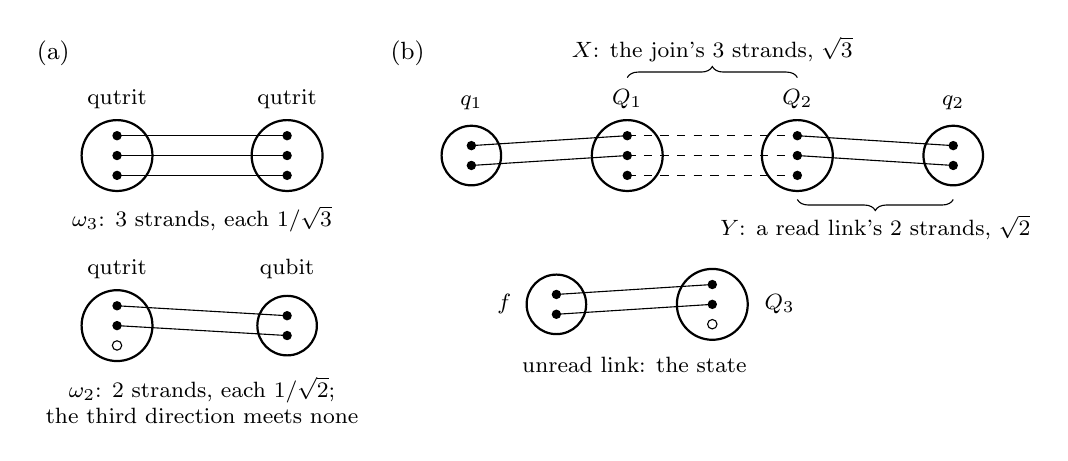
\begin{tikzpicture}[scale=0.9, every node/.style={font=\footnotesize}, dot/.style={circle, fill=black, inner sep=0pt, minimum size=3.4pt}, odot/.style={circle, draw, fill=white, inner sep=0pt, minimum size=3.4pt}]
\draw[thick] (0,0) circle (0.5);
\draw[thick] (2.4,0) circle (0.5);
\foreach \y in {0.28,0,-0.28} {\draw (0,\y) -- (2.4,\y); \node[dot] at (0,\y) {}; \node[dot] at (2.4,\y) {};}
\node at (0,0.8) {qutrit};
\node at (2.4,0.8) {qutrit};
\node at (1.2,-0.9) {$\ket{\omega_{3}}$: $3$ strands, each $1/\sqrt{3}$};
\draw[thick] (0,-2.4) circle (0.5);
\draw[thick] (2.4,-2.4) circle (0.42);
\draw (0,-2.12) -- (2.4,-2.26);
\draw (0,-2.4) -- (2.4,-2.54);
\node[dot] at (0,-2.12) {}; \node[dot] at (0,-2.4) {}; \node[odot] at (0,-2.68) {};
\node[dot] at (2.4,-2.26) {}; \node[dot] at (2.4,-2.54) {};
\node at (0,-1.6) {qutrit};
\node at (2.4,-1.6) {qubit};
\node[align=center] at (1.2,-3.45) {$\ket{\omega_{2}}$: $2$ strands, each $1/\sqrt{2}$;\\the third direction meets none};
\node[font=\small] at (-0.9,1.45) {(a)};
\draw[thick] (5,0) circle (0.42);
\draw[thick] (7.2,0) circle (0.5);
\draw[thick] (9.6,0) circle (0.5);
\draw[thick] (11.8,0) circle (0.42);
\draw (5,0.14) -- (7.2,0.28);
\draw (5,-0.14) -- (7.2,0);
\foreach \y in {0.28,0,-0.28} {\draw[dashed] (7.2,\y) -- (9.6,\y);}
\draw (9.6,0.28) -- (11.8,0.14);
\draw (9.6,0) -- (11.8,-0.14);
\foreach \y in {0.28,0,-0.28} {\node[dot] at (7.2,\y) {}; \node[dot] at (9.6,\y) {};}
\foreach \y in {0.14,-0.14} {\node[dot] at (5,\y) {}; \node[dot] at (11.8,\y) {};}
\node at (5,0.75) {$q_{1}$};
\node at (7.2,0.8) {$Q_{1}$};
\node at (9.6,0.8) {$Q_{2}$};
\node at (11.8,0.75) {$q_{2}$};
\draw[decorate, decoration={brace, amplitude=4pt}] (7.2,1.1) -- (9.6,1.1);
\node at (8.4,1.5) {$X$: the join's $3$ strands, $\sqrt{3}$};
\draw[decorate, decoration={brace, amplitude=4pt, mirror}] (9.6,-0.62) -- (11.8,-0.62);
\node at (10.7,-1.02) {$Y$: a read link's $2$ strands, $\sqrt{2}$};
\draw[thick] (8.4,-2.1) circle (0.5);
\draw[thick] (6.2,-2.1) circle (0.42);
\draw (8.4,-1.82) -- (6.2,-1.96);
\draw (8.4,-2.1) -- (6.2,-2.24);
\node[dot] at (8.4,-1.82) {}; \node[dot] at (8.4,-2.1) {}; \node[odot] at (8.4,-2.38) {};
\node[dot] at (6.2,-1.96) {}; \node[dot] at (6.2,-2.24) {};
\node[anchor=west] at (9.0,-2.1) {$Q_{3}$};
\node[anchor=east] at (5.7,-2.1) {$f$};
\node at (7.3,-2.95) {unread link: the state};
\node[font=\small] at (4.1,1.45) {(b)};
\end{tikzpicture}
\caption{The computation in strands. (a)~A pair of dimension $d$ as $d$ strands, one for each term of $\ket{\omega_{d}}$, Eq.~(\ref{eq:pair}) of the Letter, each of amplitude $1/\sqrt{d}$. A qutrit and a qubit share two strands; the qutrit's third direction (hollow) meets none. (b)~The object of Fig.~\ref{fig:link}(a) in strands, with the shared qutrit drawn as its three copies $Q_{1}$, $Q_{2}$, $Q_{3}$, one per link: the read links $q_{1}Q_{1}$ and $Q_{2}q_{2}$, two strands each; the join of $Q_{1}$ with $Q_{2}$, the qutrit pair $\ket{\omega_{3}}$, three strands (dashed); and the unread link $Q_{3}f$, which carries the state. A path from $q_{1}$ to $q_{2}$ crosses three strands, with amplitude $1/(2\sqrt{3})$, and its two paths give $\ket{\omega_{2}}_{q_{1}q_{2}}/\sqrt{6}$. Both exchanges act on the slots as the mirror of the drawing, the exchange of reads $X$ on records with both letters on ends of one kind and the exchange of links $Y$ on those with one letter at a copy and one at a qubit. A record that survives $X$ runs over the join's three strands and carries $\sqrt{3}$, the qubit--qubit records included, by the clause of Table~\ref{tab:inputs} that a read is an act at the end at which it is taken; one that survives $Y$ runs over a read link's two and carries $\sqrt{2}$. The strands are drawn in a basis; the amplitudes, counts, and weights do not depend on it.}
\label{fig:s-strands}
\end{figure}
